\documentclass[a4paper, 12pt]{article}
\usepackage[top=2cm, bottom = 2cm, left = 2cm, right = 2cm]{geometry}
\usepackage[utf8]{inputenc}
\usepackage[brazil]{babel}
\usepackage{listings}
\usepackage[framed, numbered]{matlab-prettifier}
\usepackage[T1]{fontenc}
\usepackage{indentfirst}
\usepackage{graphicx}
\usepackage{epstopdf}
\usepackage{float}
\usepackage{amsmath}
\usepackage{amssymb}
\usepackage{systeme}

\title{Relatório do Laboratório 1 - Sinais \\ EET-01}

\author{
  Igor Magalhães\\igorcmag@gmail.com
  \and
  Rafael Gonçalves\\rafael.goncalves@ga.ita.br
}
\date{23 de março de 2020}

\begin{document}
\maketitle
\section{Impulsos}

\subsection{a)}

Para gerar e plotar as quatro sequências, usamos o código 1 apresentado abaixo.

\lstinputlisting[style=Matlab-editor, caption={Código em MATLAB para gerar as quatro sequências do item (a) do exercício 1, bem como a plotagem dos seus respectivos gráficos.}, basicstyle = \mlttfamily\scriptsize]{../Programas/ex1/a.m}

Os gráficos das quatro sequências estão exibidos na figura \ref{fig:1a}, apresentada abaixo.

\begin{figure}[H]
	\centering
	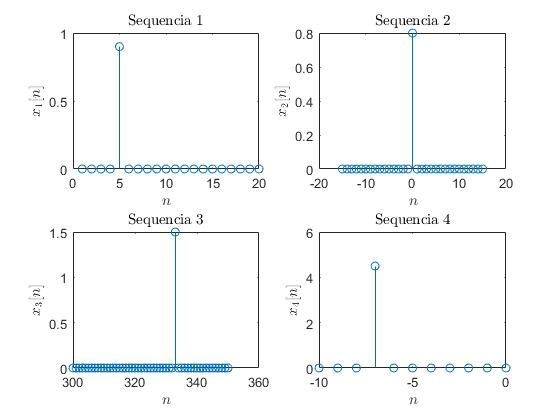
\includegraphics[scale=0.7]{../Imagens/ex1/a.jpg} 
	\caption{Gráficos das sequências em seus respectivos domínios}
	\label{fig:1a}
\end{figure}

\subsection{b)}
Para gerar e plotar o trem de impulsos, usamos o código 2 apresentado abaixo.

\lstinputlisting[style=Matlab-editor, caption={Código em MATLAB para gerar e plotar o trem de impulsos.}, basicstyle = \mlttfamily\scriptsize]{../Programas/ex1/b.m}

O gráfico obtido está na figura \ref{fig:1b}, exposta abaixo.
\begin{figure}[H]
	\centering
	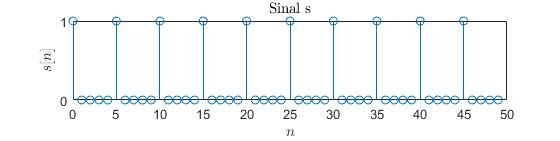
\includegraphics[scale=0.7]{../Imagens/ex1/b.jpg}  
	\caption{Gráfico do trem de impulsos}
	\label{fig:1b}
\end{figure}

\subsection{c)}

Usamos o código 3, apresentado abaixo, para gerar e plotar o vetor $x$.

\newpage

\lstinputlisting[style=Matlab-editor, caption={Criação e plotagem do vetor $x$}, basicstyle = \mlttfamily\scriptsize]{../Programas/ex1/c.m}

Obtivemos, então, o gráfico da figura \ref{fig:1c}, mostrado abaixo.

\begin{figure}[H]
	\centering
	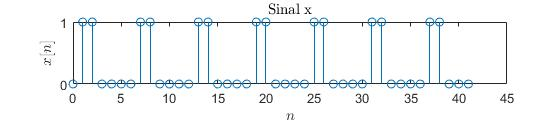
\includegraphics[scale=0.7]{../Imagens/ex1/c.jpg}  
	\caption{Gráfico do vetor $x$}
	\label{fig:1c}
\end{figure}

O vetor $x$ pode ser escrito na forma $$ x[n] = \sum_{k=0}^{P-1}\sum_{m=0}^{M-1} A_k\delta[n-k-mP] $$

com $P=6$, $M=7$ e 

\[
\begin{bmatrix}
   	A_0\\
    A_1\\
    A_2\\
    A_3\\
    A_4\\
    A_5\\
    
\end{bmatrix}
=
\begin{bmatrix}
    0\\
    1\\
    1\\
    0\\
    0\\
    0\\
\end{bmatrix}
\]

resultando em $$ x[n] = \sum_{m=0}^6\lbrace\delta[n-1-6m] + \delta[n-2-6m]\rbrace$$

\section{Sinusoides}

\subsection{a)}

Para gerar e plotar as quatro sequências, usamos o código 4 apresentado abaixo.

\lstinputlisting[style=Matlab-editor, caption={Código em MATLAB que gera as quatro sequências e plota seus respectivos gráficos}, basicstyle = \mlttfamily\scriptsize]{../Programas/ex2/a.m}

Os gráficos das sequências estão na figura \ref{fig:2a} exposta abaixo.

\begin{figure}[H]
	\centering
	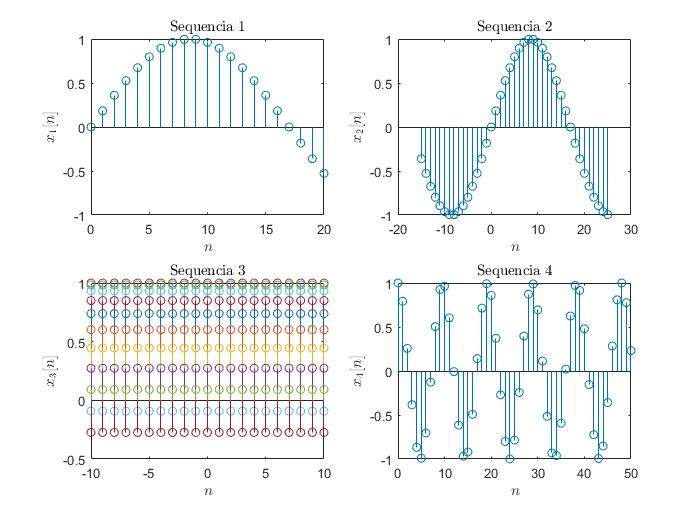
\includegraphics[scale=0.7]{../Imagens/ex2/a.jpg}  
	\caption{Gráficos das quatro sequências nos seus domínios correspondentes}
	\label{fig:2a}
\end{figure}

Uma forma simplificada de escrever $x_3[n]$ é 

$$ x_3[n]=sin(3\pi n+\frac{\pi}{2})=sin(3\pi n)cos(\frac{\pi}{2}) + cos(3\pi n)sen(\frac{\pi}{2})=cos(3\pi n)\therefore$$

\[\therefore   
x[n] = 
     \begin{cases}
       1 &\quad\text{se } n \text{ é par}\\
       -1 &\quad\text{se } n \text{ é impar}\\
     \end{cases}
\]

Além disso, a sequência $x_4$ não é periódica pois o período fundamental $P$ de um cosseno da forma $Acos(\omega t + \phi)$ é dado por 

$$P=\frac{2\pi}{\omega}$$
mas para o caso da sequência, isso resultaria num período múltiplo de $\sqrt{23}$, que nunca é inteiro.

\subsection{b)}

A função $gerarSinusoideFinita$ foi implementada com o código 5 apresentado abaixo

\lstinputlisting[style=Matlab-editor, caption={Função geradora de sinusoides finitos}, basicstyle = \mlttfamily\scriptsize]{../Programas/ex2/gerarSinusoideFinita.m}

Testamos a função para alguns conjuntos de parâmetros de entrada, bem como aquele pedido pelo enunciado (sequência 6). Isto é feito pelo código 6 mostrado abaixo.

\lstinputlisting[style=Matlab-editor, caption={Teste da função $gerarSinusoideFinita$ para alguns conjuntos de parâmetros de entrada}, basicstyle = \mlttfamily\scriptsize]{../Programas/ex2/b.m}

Os gráficos obtidos estão expostos na figura \ref{fig:2b}. 

\begin{figure}[H]
	\centering
	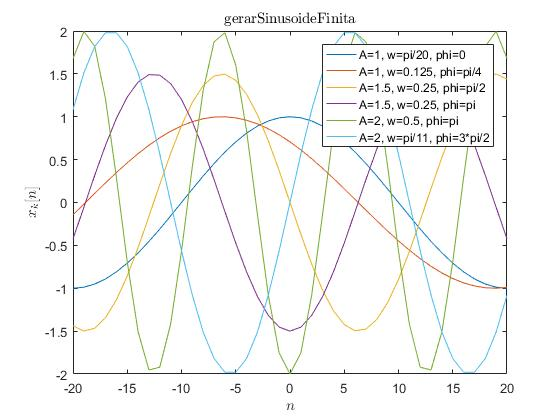
\includegraphics[scale=0.7]{../Imagens/ex2/b.jpg}  
	\caption{Gráficos das sequências geradas pela função geradora de sinusoide}
	\label{fig:2b}
\end{figure}

Neste caso, preferimos utilizar a função $plot$ do MATLAB para facilitar a visualização das ondas.

\subsection{c)}
Reescrevemos a função $gerarSinusoideFinita$ para que ela também devolvesse um vetor de índices sobre o intervalo de $n$. O código é apresentado abaixo.

\lstinputlisting[style=Matlab-editor, caption={Função $gerarSinusoideFinita2$, que agora também devolve um vetor dos índices $n$}, basicstyle = \mlttfamily\scriptsize]{../Programas/ex2/gerarSinusoideFinita2.m}

\section{Sinusoides amostrados}

\subsection{a)}
Utilizamos o código abaixo para criar a função $sinusoidesAmostradas$, que amostra um sinal sinusoidal

\newpage

\lstinputlisting[style=Matlab-editor, caption={Função $sinusoidesAmostradas$}, basicstyle = \mlttfamily\scriptsize]{../Programas/ex3/sinusoidesAmostradas.m}

Utilizamos a função $sinusoidesAmostradas$ para amostrar o sinal descrito pelo enunciado, conforme o código abaixo.

\lstinputlisting[style=Matlab-editor, caption={Plotagem dos gráficos em função do tempo e do índice}, basicstyle = \mlttfamily\scriptsize]{../Programas/ex3/a.m}

O gráfico obtido em função do tempo foi

\begin{figure}[H]
	\centering
	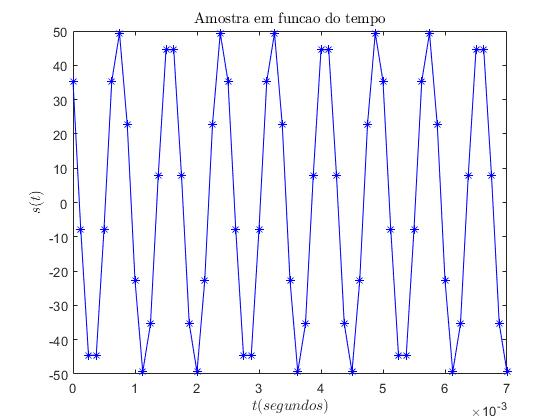
\includegraphics[scale=0.7]{../Imagens/ex3/a1.jpg}  
	\caption{Gráfico da amostra em função do tempo}
	\label{fig:3a1}
\end{figure}

e o gráfico obtido em função do índice foi

\begin{figure}[H]
	\centering
	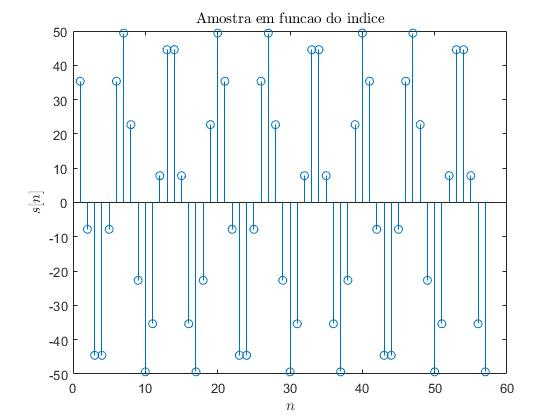
\includegraphics[scale=0.7]{../Imagens/ex3/a2.jpg}  
	\caption{Gráfico da amostra em função do índice}
	\label{fig:3a2}
\end{figure}

O sinal discreto resultante tem comprimento 57 e possui 8 períodos incluídos.

\subsection{b)}
Se $t_n = nT=\frac{n}{f_0}$ e $\phi=\frac{3\pi}{2}$, então 
$$s(t_n)=s[n]=Acos(2\pi f_0t_n+\phi)=Acos(2\pi n + \phi)=Asen(2\pi n),$$
que é uma onda senoidal.

Utilizamos o código 10 para gerar uma onda senoidal discreta, começando em $t=5s$ e terminando em $t=15s$. Para isso apenas precisamos inserir uma fase inicial $\phi=\frac{3\pi}{2}$. A onda é da forma $30sin(0.4\omega t)$.

\lstinputlisting[style=Matlab-editor, caption={Gerando uma onda senoidal discreta}, basicstyle = \mlttfamily\scriptsize]{../Programas/ex3/b.m}

O gráfico obtido está apresentado na figura 8.
\begin{figure}[H]
	\centering
	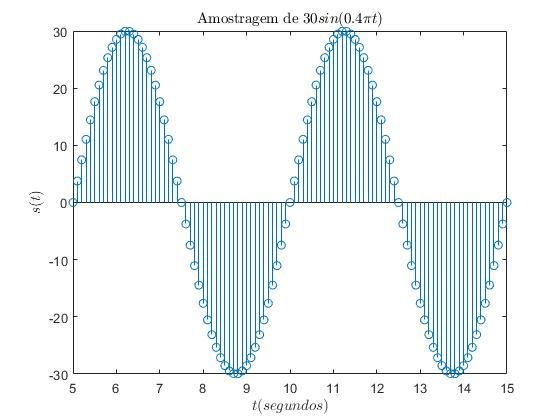
\includegraphics[scale=0.7]{../Imagens/ex3/b.jpg}  
	\caption{Gráfico de uma onda senoidal discreta}
	\label{fig:3b}
\end{figure}

\section{Exponenciais complexos}

\subsection{a)}

$$z_0=0,9\angle45^{o}=0,9e^{j\frac{\pi}{4}} \therefore x[n]=z_0^n=0,9^ne^{j\frac{\pi}{4}n}=0,9^n(cos(\frac{\pi}{4}n) + jsin(\frac{\pi}{4}n))$$
$$Re(x[n]) = 0,9^ncos(\frac{\pi}{4}n) \text{ e } Im(x[n]) = 0,9^nsin(\frac{\pi}{4}n)$$

O código 11 foi utilizado para implementar a exponencial complexa, bem como os gráficos de sua parte real e imaginária.

\lstinputlisting[style=Matlab-editor, caption={Implementação e gráficos da exponencial complexa}, basicstyle = \mlttfamily\scriptsize]{../Programas/ex4/a.m}

Os gráficos obtidos estão na figura \ref{fig:4a}.

\begin{figure}[H]
	\centering
	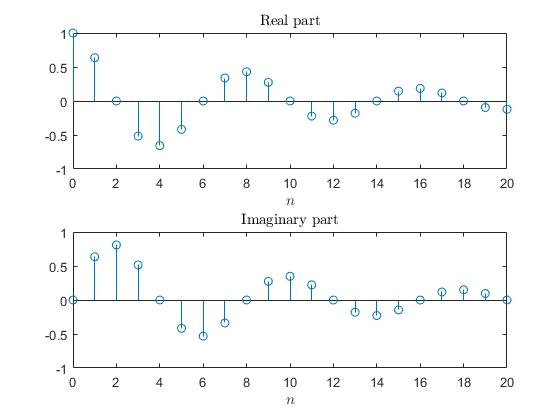
\includegraphics[scale=0.7]{../Imagens/ex4/a.jpg}  
	\caption{Parte real e parte imaginária da exponencial complexa}
	\label{fig:4a}
\end{figure}

\subsection{b)}

No código 12, fizemos gráficos da parte imaginária pela parte real para alguns valores de $\theta$. A sequência do item (a) é a terceira sequência ($\theta=\frac{\pi}{4}$).

\lstinputlisting[style=Matlab-editor, caption={teste}, basicstyle = \mlttfamily\scriptsize]{../Programas/ex4/b.m}

Os gráficos obtidos estão na figura \ref{fig:4b}.

\begin{figure}[H]
	\centering
	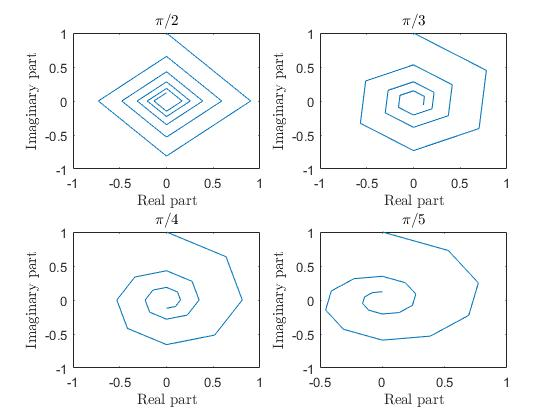
\includegraphics[scale=0.7]{../Imagens/ex4/b.jpg}  
	\caption{Parte imaginária versus parte real para alguns valores de $\theta$}
	\label{fig:4b}
\end{figure}

\subsection{c)}

Para $z_k[n]=A_kr_k^ncos(\theta_k n + \phi_k) + jsen(\theta_k n + \phi_k)$, temos

$$
A = \begin{bmatrix}
   	3\\
    1\\
    1\\
    1\\
    \end{bmatrix}
\text{ , } 
r = \begin{bmatrix}
   	1\\
    1\\
    1,1\\
    0,9\\
    \end{bmatrix} 
\text{ , } 
\theta = \begin{bmatrix}
   	-\frac{\pi}{7}\\
    -\frac{\pi}{17}\\
    \frac{\pi}{11}\\
    \frac{\pi}{11}\\
    \end{bmatrix}  
\text{ e } 
\phi = \begin{bmatrix}
   	\frac{\pi}{2}\\
    \frac{\pi}{2}\\
    \frac{\pi}{4}\\
    0\\
    \end{bmatrix} 
$$

Implementamos as sequência e obtivemos seus gráficos através do código 13.

\lstinputlisting[style=Matlab-editor, caption={Implementação e plotagem das quatro exponenciais complexas}, basicstyle = \mlttfamily\scriptsize]{../Programas/ex4/c.m}

Os gráficos obtidos estão expostos na figura \ref{fig:4c}

\begin{figure}[H]
	\centering
	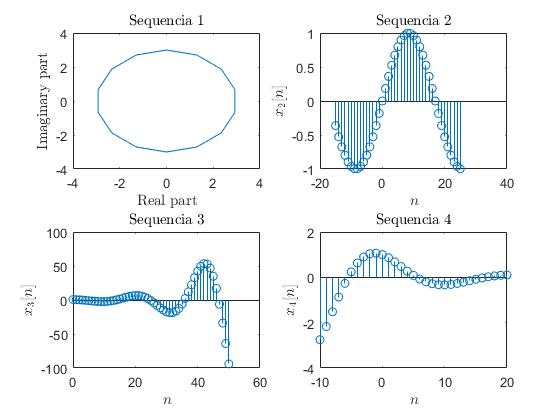
\includegraphics[scale=0.7]{../Imagens/ex4/c.jpg}  
	\caption{Gráficos das exponenciais complexas. Somente a sequência 1 possui parte real e parte imaginária. As demais possuem apenas parte real.}
	\label{fig:4c}
\end{figure}

\end{document}